\documentclass[letterpaper, 12pt]{math}

\usepackage{tikz}

\title{University Physics 1A}
\author{Alvin Lin}
\date{September 28th, 2017}

\begin{document}

\maketitle

\section*{Air resistance}
One model of air resistance:
\[ F_{air} = K_1v^2 \]
This model has many common everyday uses. Another model uses a constant for
\( K_2 \) depending on the size, shape, and other properties of the
object.
\[ F_{air} = K_2v \]
For a falling object:
\[ F_{net} = F_{air}-mg \]
For some \( v \), \( F_{air}-mg = 0 \), which means the acceleration is 0. This
is the point at which the object has reached ``terminal velocity''.
\[ K_1v^2-mg = 0 \]
\[ v^2 = \frac{mg}{K_1} \]

\subsection*{Practice Problem}
A ball of mass 1.34kg is attached to a vertical rod by two strings. The top
string is 1.60m long and makes a \( 30.0^{\circ} \) angle with the rod, while
the bottom string makes a \( 45.06^{\circ} \) angle with the rod. The rod is
rotated at 1 revolution every 1.20s. Find the tension in each string.
\begin{center}
  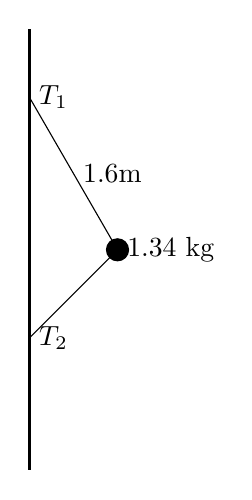
\begin{tikzpicture}[scale=1.4]
    \draw[fill] (0,0) circle (0.1cm);
    \draw (0,0) node[right] {1.34 kg} -- node[pos=0.5, right] {1.6m}
      (-0.8,1.385) node[right] {\( T_1 \)};
    \draw (0,0) -- (-0.8,-0.8) node[right] {\( T_2 \)};
    \draw[very thick] (-0.8,2) -- (-0.8,-2);
  \end{tikzpicture}
\end{center}
Free body diagram:
\begin{center}
  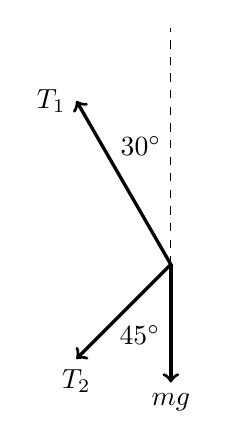
\begin{tikzpicture}[scale=1.5]
    \draw[->, very thick] (0,0) -- (-0.8,1.385) node[left] {\( T_1 \)};
    \draw[dashed] (0,0) -- node[pos=0.5, left] {\( 30^{\circ} \)} (0,2);
    \draw[->, very thick] (0,0) -- (-0.8,-0.8) node[below] {\( T_2 \)};
    \draw[->, very thick] (0,0) -- node[pos=0.6, left] {\( 45^{\circ} \)} (0,-1)
      node[below] {\( mg \)};
  \end{tikzpicture}
\end{center}
\begin{align*}
  \frac{1rev}{1.2s} &= \frac{2\pi r}{1.2s} \\
  &= 4.189\frac{m}{s} \\
\end{align*}
Horizontal net force:
\begin{align*}
  -T_1\sin(30)-T_2\sin(45) &= ma_x = -m\frac{v^2}{r} \\
  T_1\sin(30)+T_2\sin(45) &= 29.39N
\end{align*}
Vertical net force:
\begin{align*}
  T_1\cos(30)-T_2\cos(45)-mg &= ma_y = 0 \\
  T_1\cos(30)-T_2\cos(45) &= 13.13N
\end{align*}
Solving for the system of equations:
\begin{align*}
  T_1 &= 31.1N \\
  T_2 &= 19.5N
\end{align*}

\section*{Reminders and Homework}
Complete the homework on TheExpertTA and WebAssign. \\
\textbf{Remember to bring the Activities Manual.} \\

\begin{center}
  You can find all my notes at \url{http://omgimanerd.tech/notes}. If you have
  any questions, comments, or concerns, please contact me at
  alvin@omgimanerd.tech
\end{center}

\end{document}
